\smalltitle{سوال 5}
\begin{enumerate}
    \item \begin{enumerate}
        \item تمام کد‌ها اعداد تصادفی یکسانی تولید می‌کنند (به علت \lr{srand(1)})
        و در تمامی آن‌ها صرفا تمام اعداد تصادفی را با هم جمع می‌زنیم.

        اما کمی تفاوت‌های جزئی وجود دارد. مثلا در فایل
        \lr{branch\_with\_true}
        صرفا شرط جمع یا ضرب در یک تابع جداگانه تعریف شده است که همیشه 1 را برگرداند. یا مثلا در فایل
        \lr{no\_branch}
        به صورت کلی شرط را برداشته‌ایم و همیشه جمع انجام می‌شود. در فایل
        \lr{real\_branch}
        باید دقت کنیم که خروجی تابع rand همیشه یک عدد مثبت است.
        پس تمامی اعداد آرایه برابر 1 هستند و شرط همیشه برقرار است.

        فرق این فایل با فایل اول این است که زمانی که کامپایلر می‌خواهد که کد را
        optimize
        بکند به کمک \lr{static analysis}
        نمی‌تواند شرط را حذف بکند و شرط همیشه وجود دارد.
        \item برای هر کدام از فایل‌ها دستور
        \lr{sudo perf stat ./*.out}
        را زدم. نتایج به صورت زیر هستند:
        \begin{latin}
        \begin{itemize}
            \item no\_branch.out
            \begin{figure}[H]
                \centerline{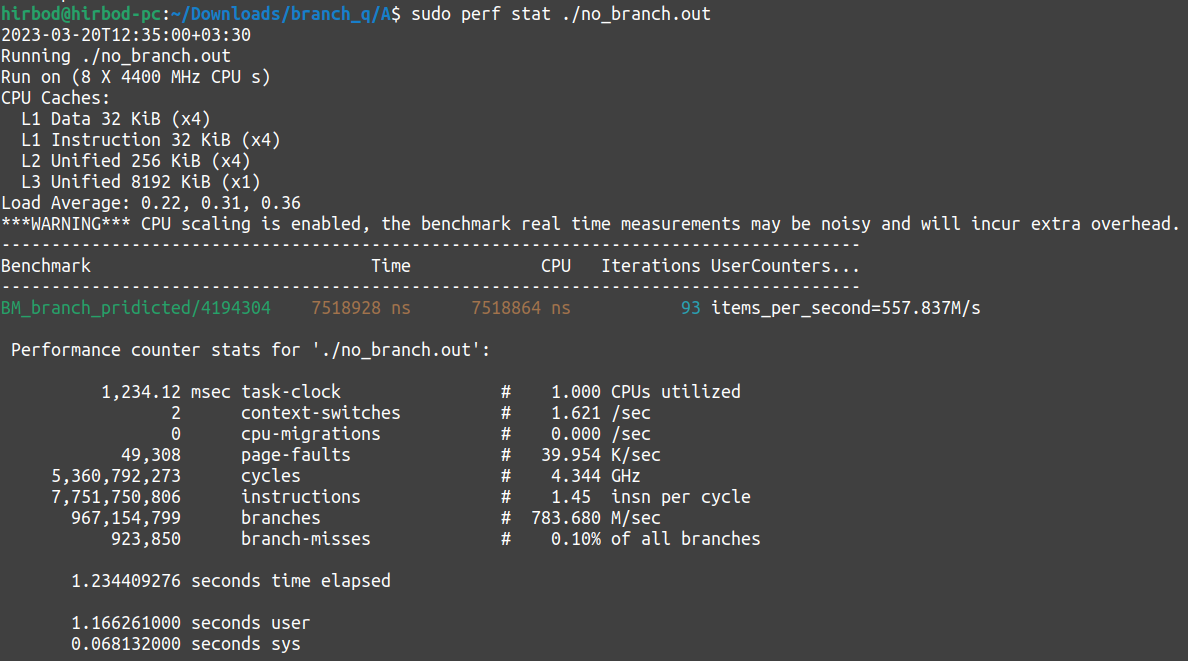
\includegraphics[scale=0.35]{pics/5/A/no_branch.png}}
            \end{figure}
            \item branch\_with\_true.out
            \begin{figure}[H]
                \centerline{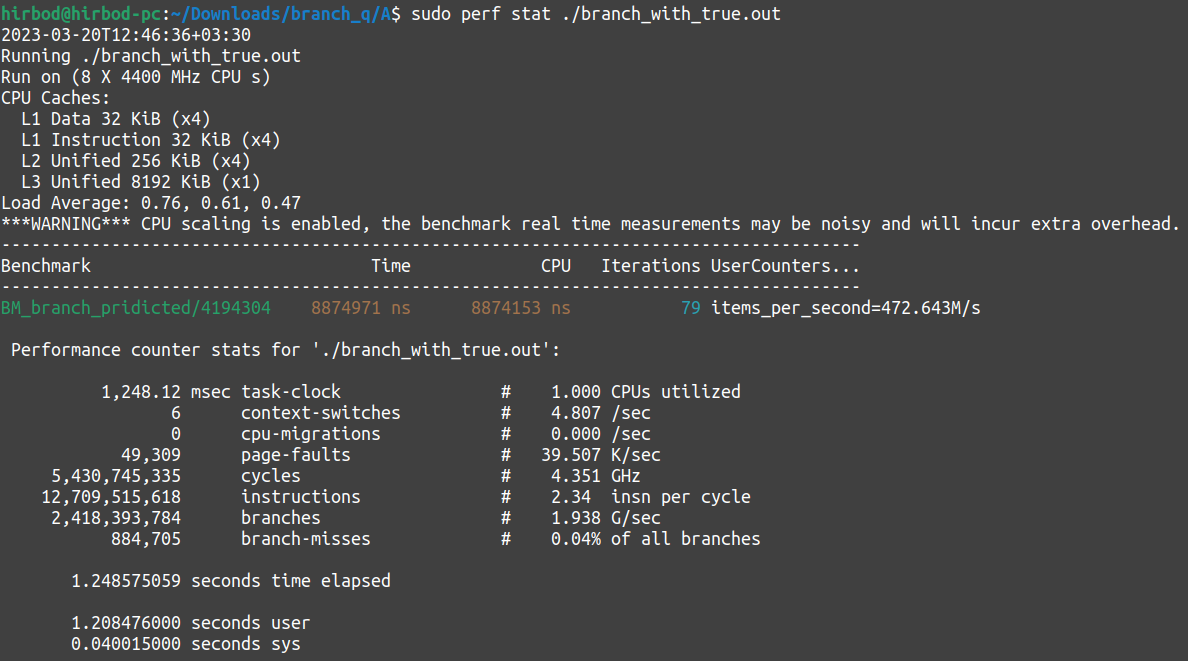
\includegraphics[scale=0.35]{pics/5/A/branch_with_true.png}}
            \end{figure}
            \item real\_branch.out
            \begin{figure}[H]
                \centerline{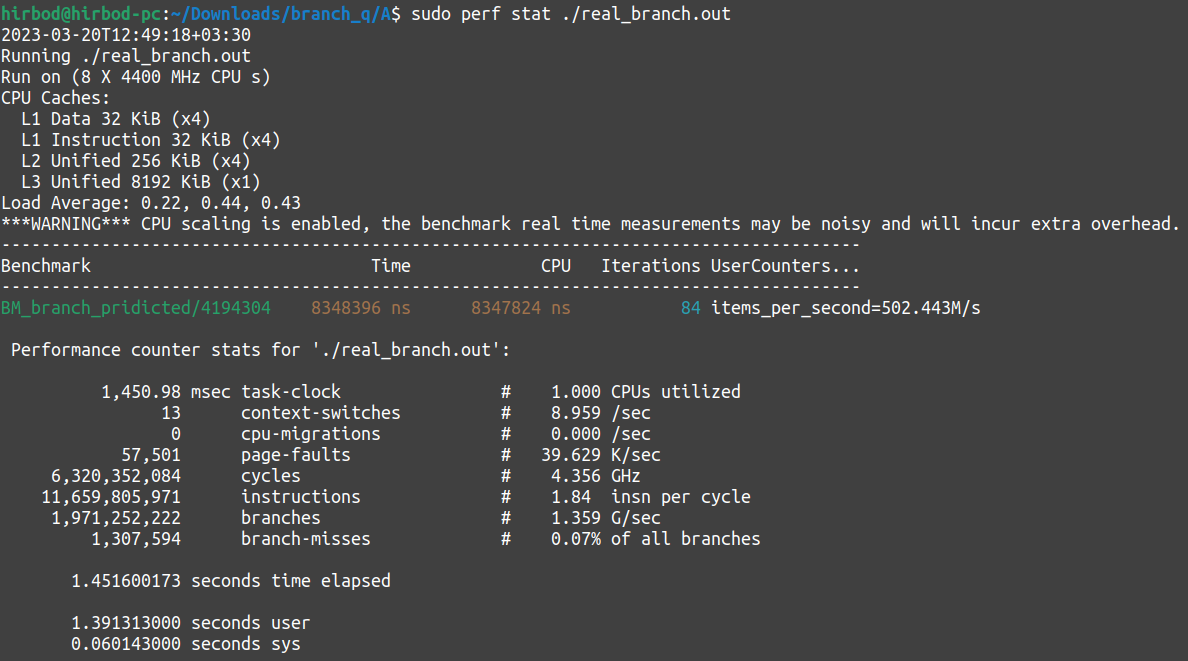
\includegraphics[scale=0.35]{pics/5/A/real_branch.png}}
            \end{figure}
        \end{itemize}
        \end{latin}
        همان طور که مشخص بود کدی که کلا branch ندارد سریع تر عمل می‌کند.
        اما کد‌هایی که branch دارند نیز به نسبت سریع هستند. همان طور که پیدا است به خاطر \lr{branch predictor cpu}
        است که این اتفاق می‌افتد. در صورتی که به نتایج perf نگاه کنیم متوجه می‌شویم که درصد خیلی کمی از
        \lr{branch}ها \lr{miss}
        شده‌اند. اما حال سوال پیش می‌آید که چرا
        \lr{branch\_with\_true}
        سریع‌تر از
        \lr{real\_branch}
        است. دلیل این موضوع را می‌توان در تعداد کل \lr{branch}ها
        مشاهده کرد. تعداد \lr{branch}های
        \lr{branch\_with\_true}
        بیشتر است. این اتفاق برای این می‌افتد که یک jump هم برای صدا زدن تابع \lr{true\_giver}
        و یک jump هم برای برگشت نیاز داریم.
        برای نگاه کردن به اسمبلی فایل من در ابتدا به کمک \lr{g++} \lr{object file}ها را ساختم و
        در ادامه به کمک
        \lr{ghidra}
        اسمبلی فایل‌ها را نگاه کردم. این اسمبلی برنامه‌ی
        \lr{brach\_with\_true}
        است:
        \begin{figure}[H]
            \centerline{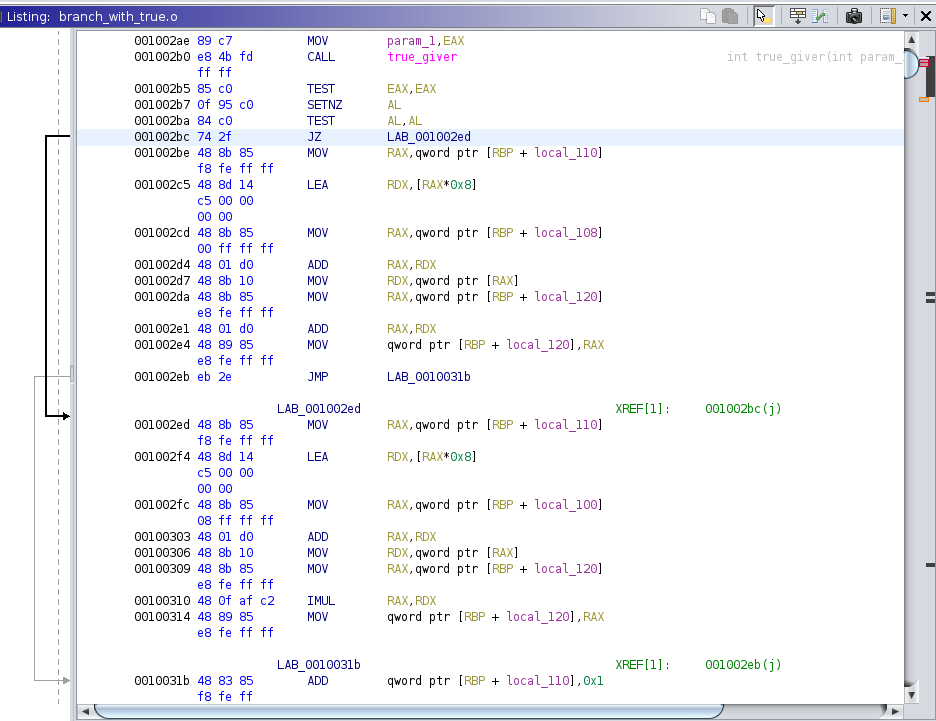
\includegraphics[scale=0.4]{pics/5/A/ghidra_branch_with_true.png}}
        \end{figure}
        و این نیز اسمبلی برنامه
        \lr{real\_branch}
        است:
        \begin{figure}[H]
            \centerline{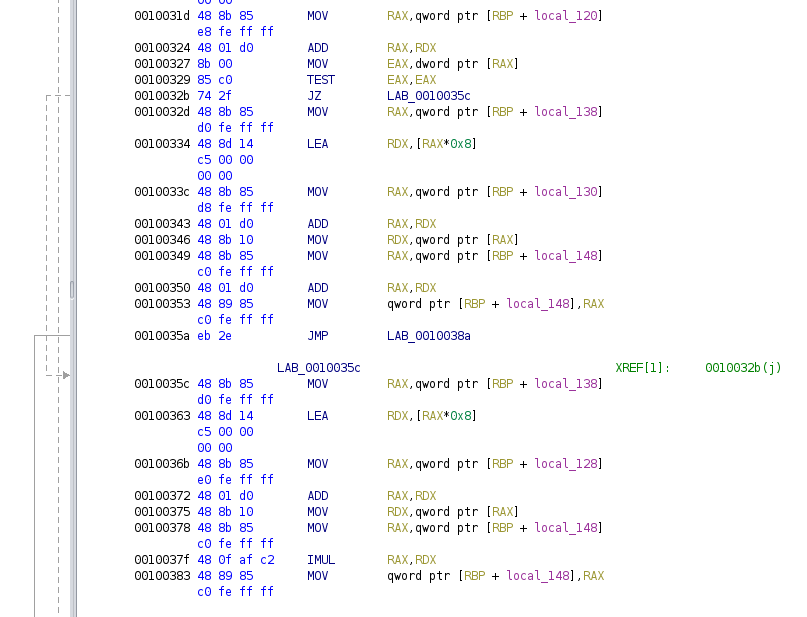
\includegraphics[scale=0.4]{pics/5/A/ghidra_real_branch.png}}
        \end{figure}
        همان طور که مشخص است تفاوت صرفا سر این است که یک call در برنامه‌ی \lr{branch\_with\_true}
        صورت گرفته است.
        \item در ابتدا صرفا هر کدام از برنامه‌ها را ران می‌کنیم:
        \begin{latin}
        \begin{itemize}
            \item no\_branch.O3
            \begin{figure}[H]
                \centerline{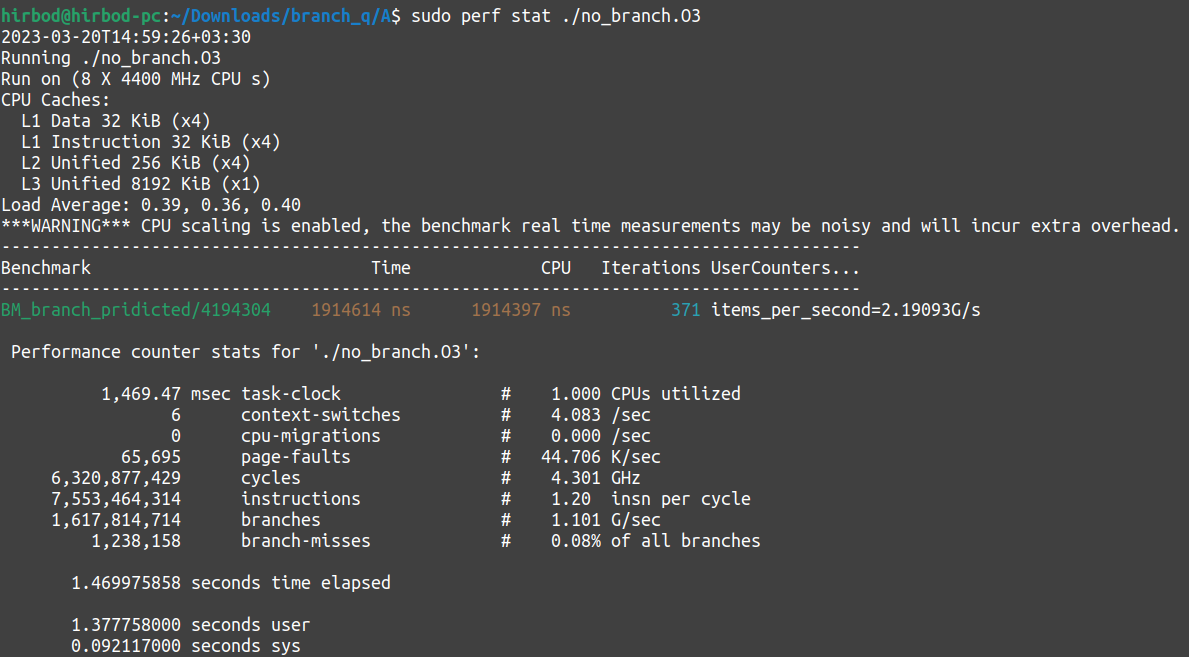
\includegraphics[scale=0.35]{pics/5/A/no_branch_o3.png}}
            \end{figure}
            \item branch\_with\_true.O3
            \begin{figure}[H]
                \centerline{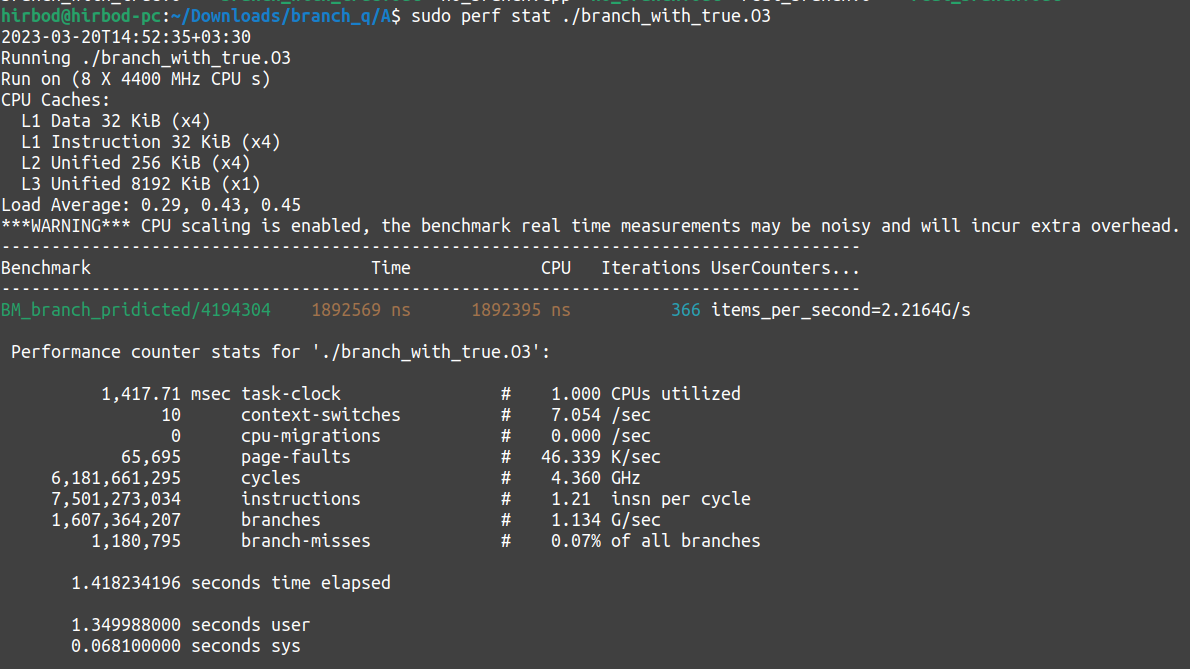
\includegraphics[scale=0.35]{pics/5/A/branch_with_true_o3.png}}
            \end{figure}
            \item real\_branch.O3
            \begin{figure}[H]
                \centerline{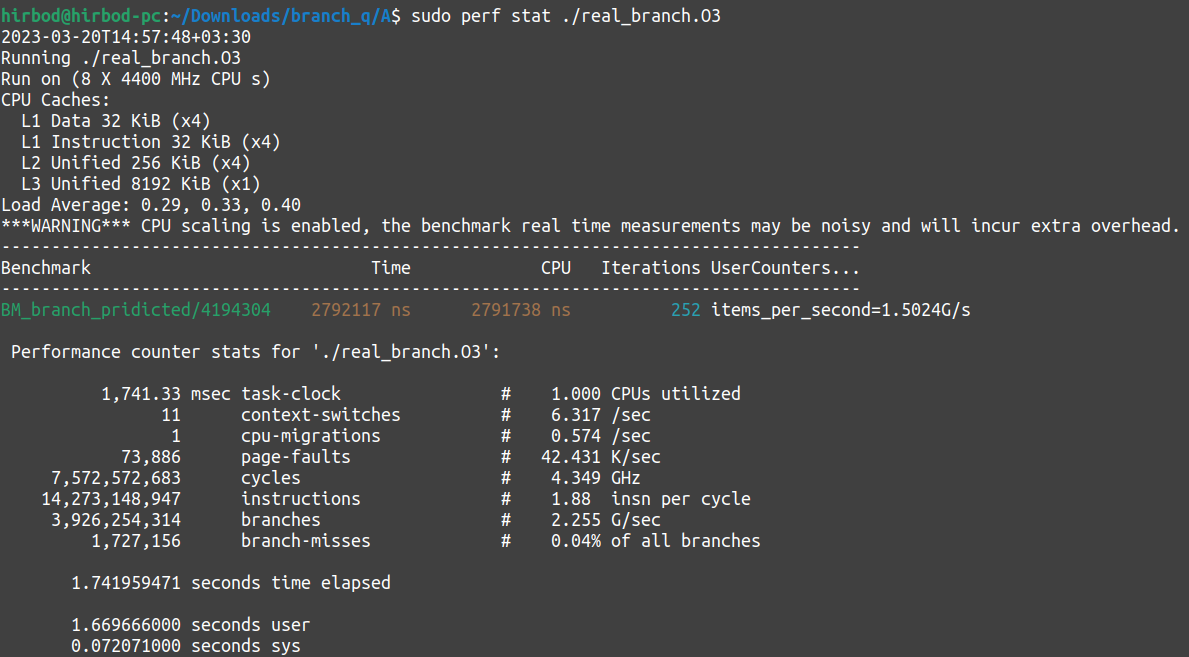
\includegraphics[scale=0.35]{pics/5/A/real_branch_o3.png}}
            \end{figure}
        \end{itemize}
        \end{latin}
        دلیل این موضوع این است که کامپایلر متوجه می‌شود که همیشه شرط موجود درست است و همیشه
        قطعه کد اول ران می‌شود. پس کامپایلر عملا شرط را بر می‌دارد و کد حاصل شبیه کد
        \lr{no\_branch}
        می‌شود. همان طور که در perf نیز مشخص است تعداد \lr{branch}ها تقریبا یکسان است.

        همچنین این تسریع سرعت را در \lr{real\_branch} نداشتیم چرا که در \lr{real\_branch}
        کامپایلر در زمان اجرا نمی‌تواند تشخیص دهد که آیا واقعا تمامی آرایه‌ی $c$
        برابر یک است یا خیر. برای همین هر دو قسمت شرط را قرار می‌دهد و یک branch اتفاق می‌افتد.
        این موضوع را می‌توان از خروجی perf نیز مشاهده کرد که تعداد \lr{branch}ها بسیار بیشتر از تعداد
        آنها در دو برنامه‌ی دیگر است.

        در نهایت نیز به کمک سایت
        \link{https://godbolt.org/}{godbolt}
        فرضیه‌ی خود را تست می‌کنیم.
        \begin{figure}[H]
            \centerline{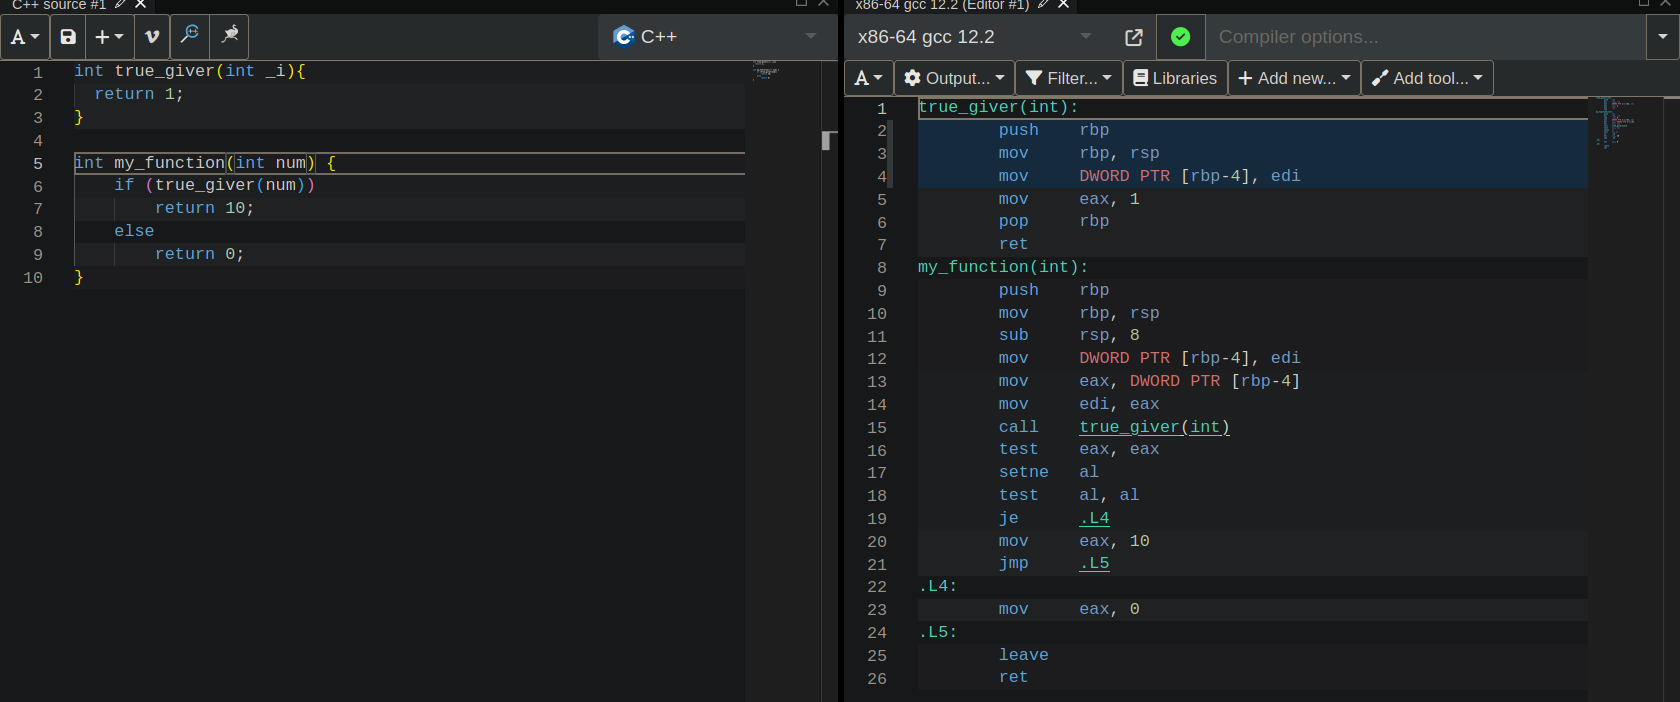
\includegraphics[scale=0.3]{pics/5/A/godbolt_o0.png}}
            \centerline{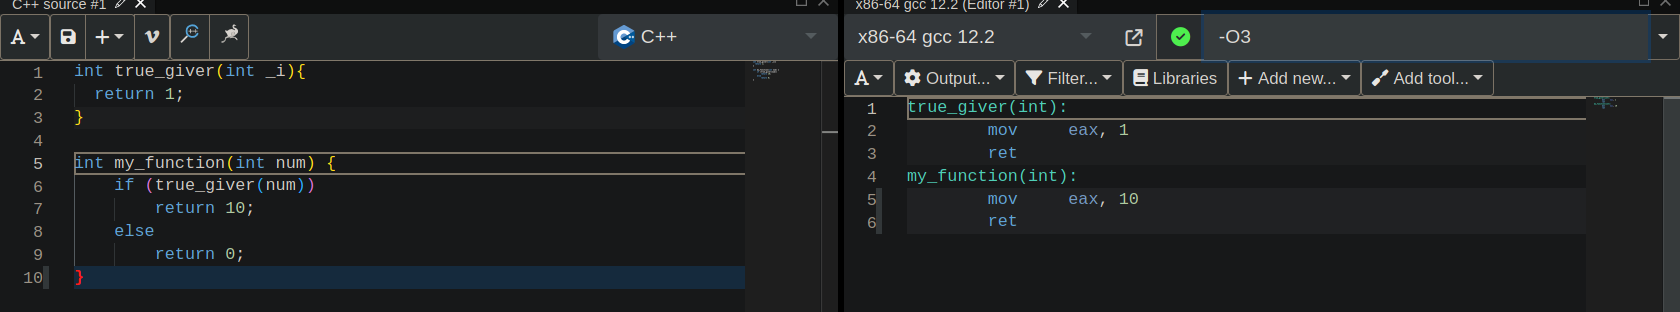
\includegraphics[scale=0.3]{pics/5/A/godbolt_o3.png}}
        \end{figure}
        همان طور که مشاهده می‌شود زمانی که از \lr{-O3}
        استفاده می‌کنیم به صورت کلی شرط برداشته می‌شود!
    \end{enumerate}
    \item فایل \lr{always\_true} همیشه شرطش درست است.
    فایل \lr{branch\_0101} یکی در میان شرط‌ها اجرا می‌شوند و نمی‌شوند.
    فایل \lr{pure\_random} کاملا تصادفی است.

    حال فایل‌ها را اجرا می‌کنیم. نتیجه‌ی \lr{perf stat} تمامی فایل‌ها را می‌توانید در زیر مشاهده کنید:
    \begin{latin}
    \begin{itemize}
        \item always\_true
        \begin{figure}[H]
            \centerline{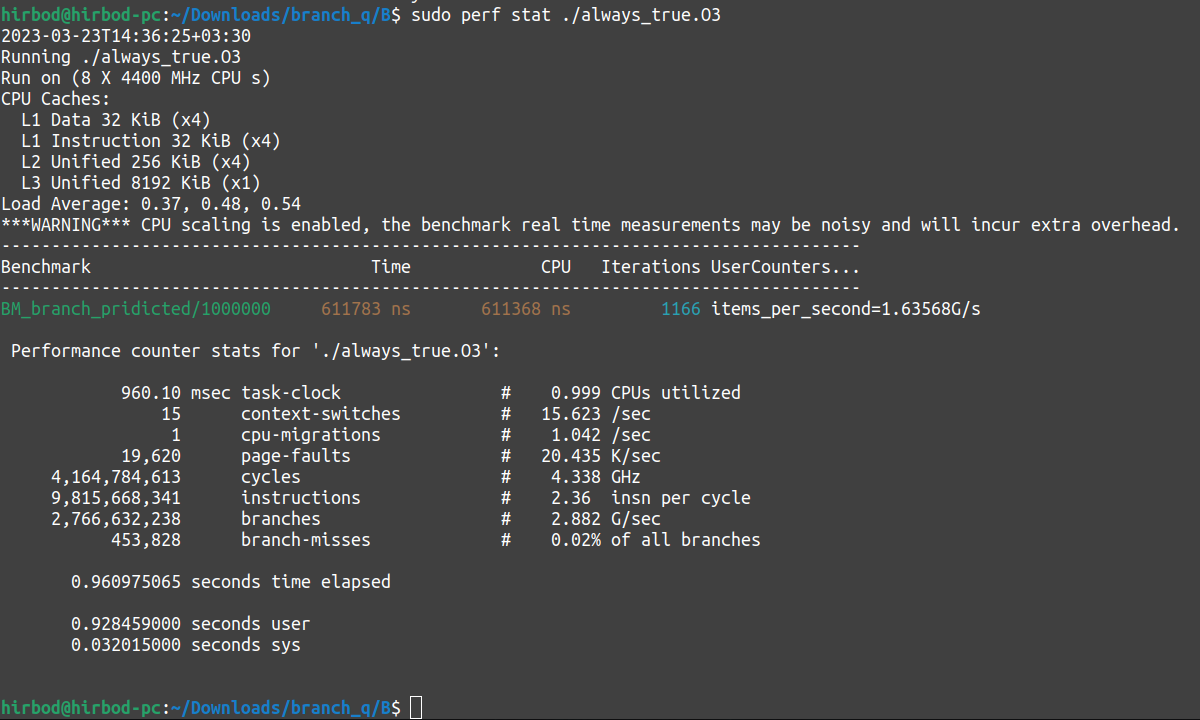
\includegraphics[scale=0.35]{pics/5/B/always_true.png}}
        \end{figure}
        \item pure\_random
        \begin{figure}[H]
            \centerline{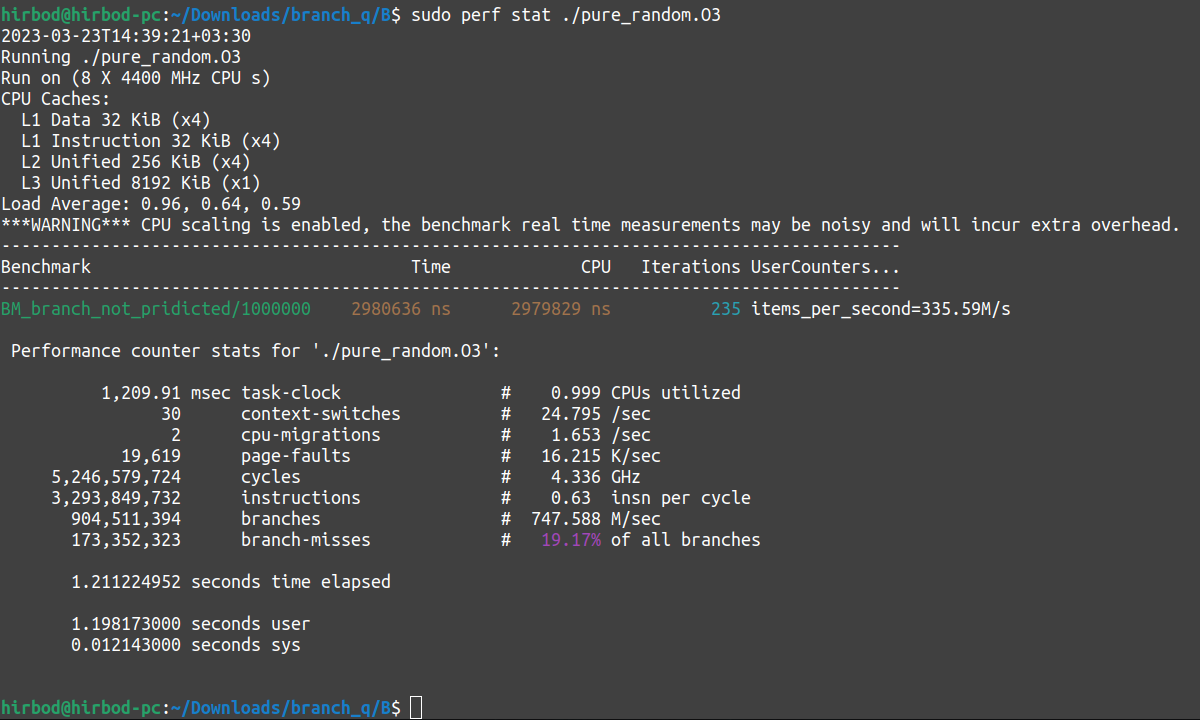
\includegraphics[scale=0.35]{pics/5/B/pure_random.png}}
        \end{figure}
        \item branch\_0101
        \begin{figure}[H]
            \centerline{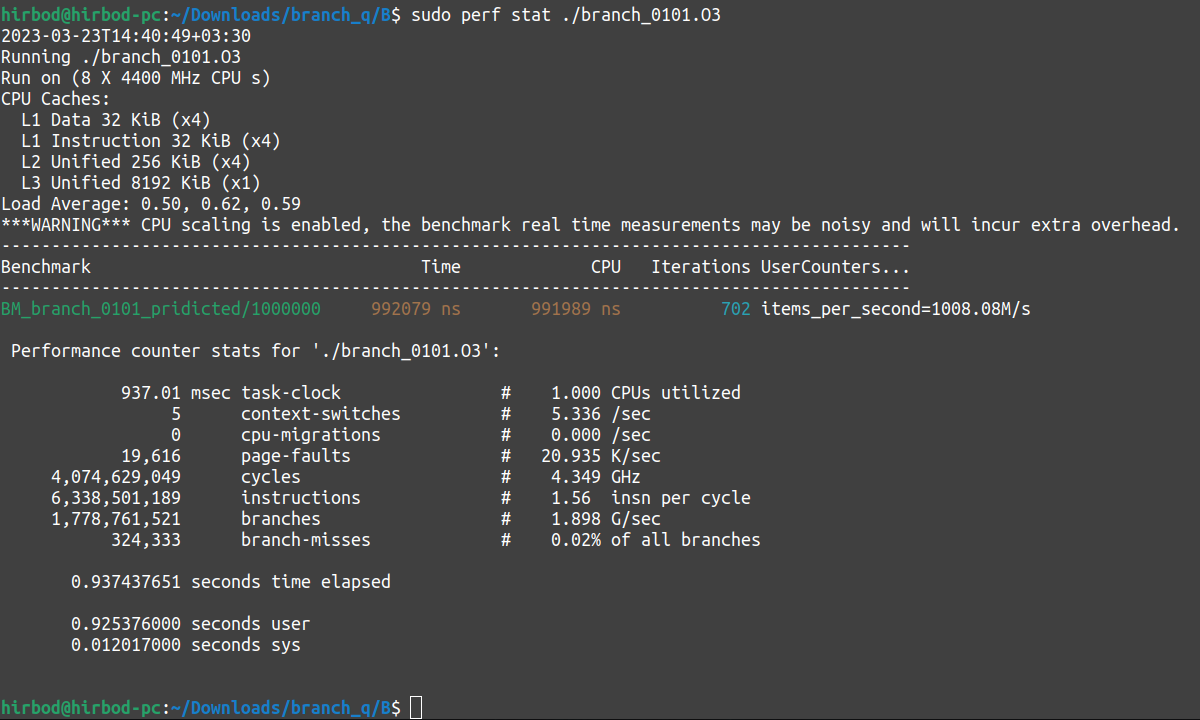
\includegraphics[scale=0.35]{pics/5/B/branch_0101.png}}
        \end{figure}
    \end{itemize}
    \end{latin}
    همان طور که مشاهده می‌کنید CPU نمی‌تواند رفتار branch در فایل
    \lr{pure\_random}
    را پیش بینی کند پس \lr{miss ratio} بسیار بالا می‌رود.

    برای بررسی رفتار perf از تکنیک کلاسیک \lr{binary search} استفاده کردم.
    فایل \lr{pure\_random.cpp} را کپی کردم در فایل \lr{semi\_random.cpp} و خط مقدار دهی $C$
    را به صورت زیر عوض کردم:
    \codesample{codes/5B-Changed.cpp}
    با این کار یک سوم اول \lr{branch}ها به صورت رندوم هستند و بقیه به صورت یکنواخت ۰ هستند.
    دوباره perf را اجرا می‌کنیم:
    \begin{figure}[H]
        \centerline{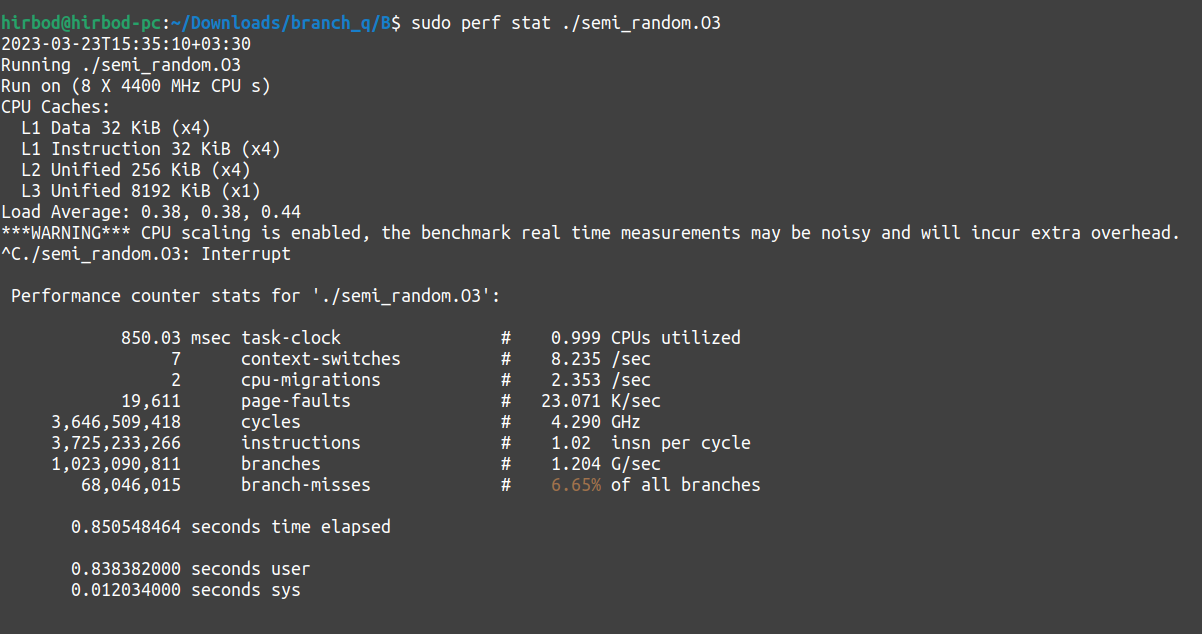
\includegraphics[scale=0.3]{pics/5/B/semi-random-yellow.png}}
    \end{figure}
    پس با زیر ۱۰ درصد \lr{branch miss} رنگ ما زرد می‌شود.
    همچنین با کمی بیشتر ور رفتن با عدد 3 در قطعه کد بالا می‌توان درصد‌های دیگر را نیز بررسی کرد. 
    با این کار می‌توان نتیجه گرفت که درصد زیر 5 برای perf طبیعی هست چرا که رنگی نمی‌شود.
    \begin{figure}[H]
        \centerline{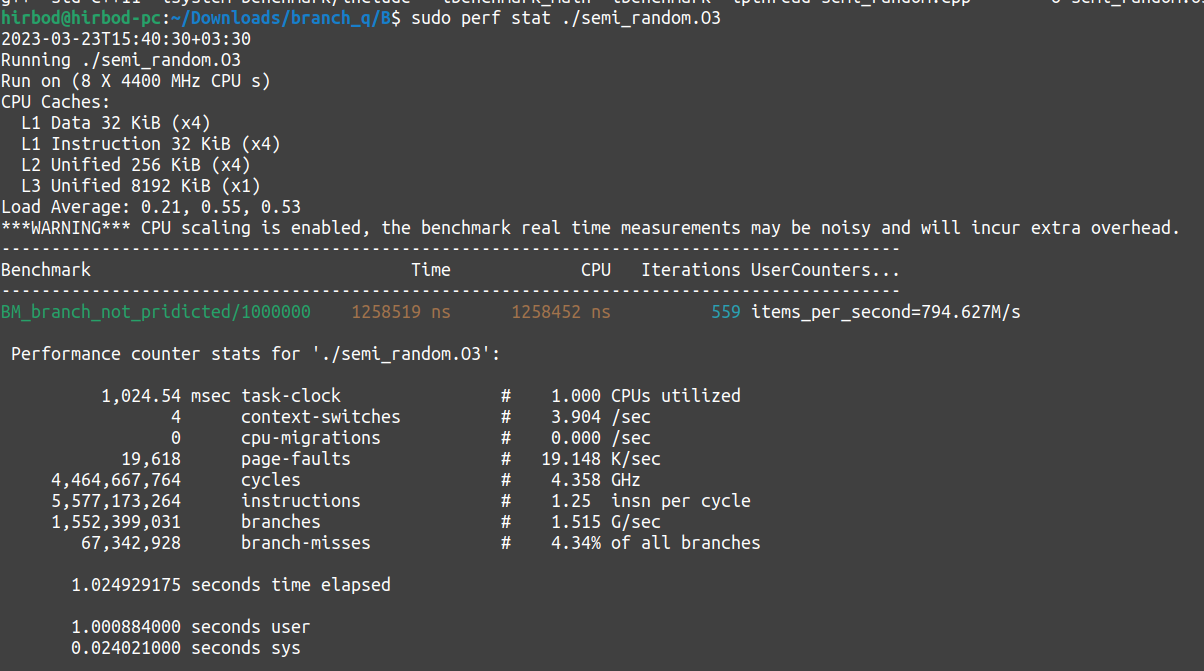
\includegraphics[scale=0.3]{pics/5/B/semi-random-white.png}}
    \end{figure}

    حال به بررسی رفتار \lr{branch\_0101} می‌پردازیم.
    همان طور که در لاگ خروجی \lr{google benchmark} مشخص است به ترتیب
    1166 و 702
    بار حلقه‌ی \lr{state}
    اجرا شده است. پس برای تعداد \lr{miss}ها داریم:
    \begin{gather*}
        \text{True Always} = \frac{453828}{1166} \approx 389.21\\
        \text{Toggling} = \frac{324333}{702} \approx 462.012
    \end{gather*}
    
    در نهایت تمامی برنامه‌ها را تحلیل می‌کنیم. مشخص است که برنامه‌ای که به صورت کلی همیشه 1 به عنوان شرطش
    است باید بیشترین سرعت و کمترین \lr{miss prediction} را داشته باشد که بدین صورت است. همچنین
    برنامه‌ای که به صورت کاملا تصادفی بین \lr{taken} و \lr{non taken} جا به جا می‌شود بدترین سرعت را داشته باشد
    چرا که نیاز به \lr{flush pipeline} زیادی به خاطر \lr{miss prediction} داریم.
    اما در صورتی که به برنامه‌ی \lr{branch\_0101} نگاه کنیم متوجه می‌شویم که آنقدر هم سرعت ما بدتر نشده است.
    این موضوع به خاطر این است که \lr{CPU}های امروزی یک جور حافظه برای
    ذخیره کردن و به یاد سپردن الگو‌ها در \lr{branch}ها را دارند.
    می‌توانید برای اطلاعات بیشتر و در آوردن مقدار این حافظه
    \link{https://stackoverflow.com/a/55440106}{این}
    لینک را مطالعه کنید.
    \item در این دو فایل یک فایل که از قسمت قبل آمده است که همه‌ی عضو‌های آرایه‌ی $C$ برابر ۱ هستند
    چرا که خروجی \lr{rand} همیشه از ۰ بزرگتر مساوی است. از طرفی در فایل دیگر آرایه‌ی $C1$
    به صورت رندوم مقدار دهی می‌شود ولی متمم آن در $C2$
    ذخیره می‌شود. در زمان بررسی شرط عملا
    $a \vee \sim a$
    بررسی می‌شود که همیشه درست است. حال perf را اجرا می‌کنیم.
    \begin{latin}
    \begin{itemize}
        \item always\_true
        \begin{figure}[H]
            \centerline{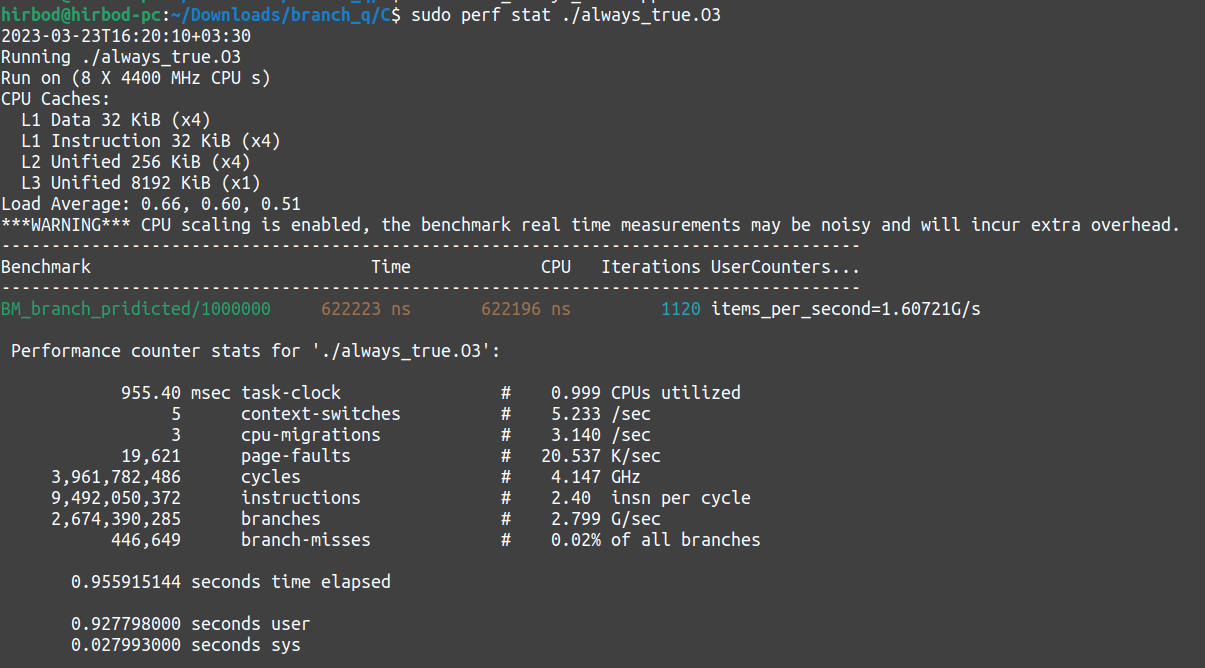
\includegraphics[scale=0.35]{pics/5/C/always_true.png}}
        \end{figure}
        \item also\_always\_true
        \begin{figure}[H]
            \centerline{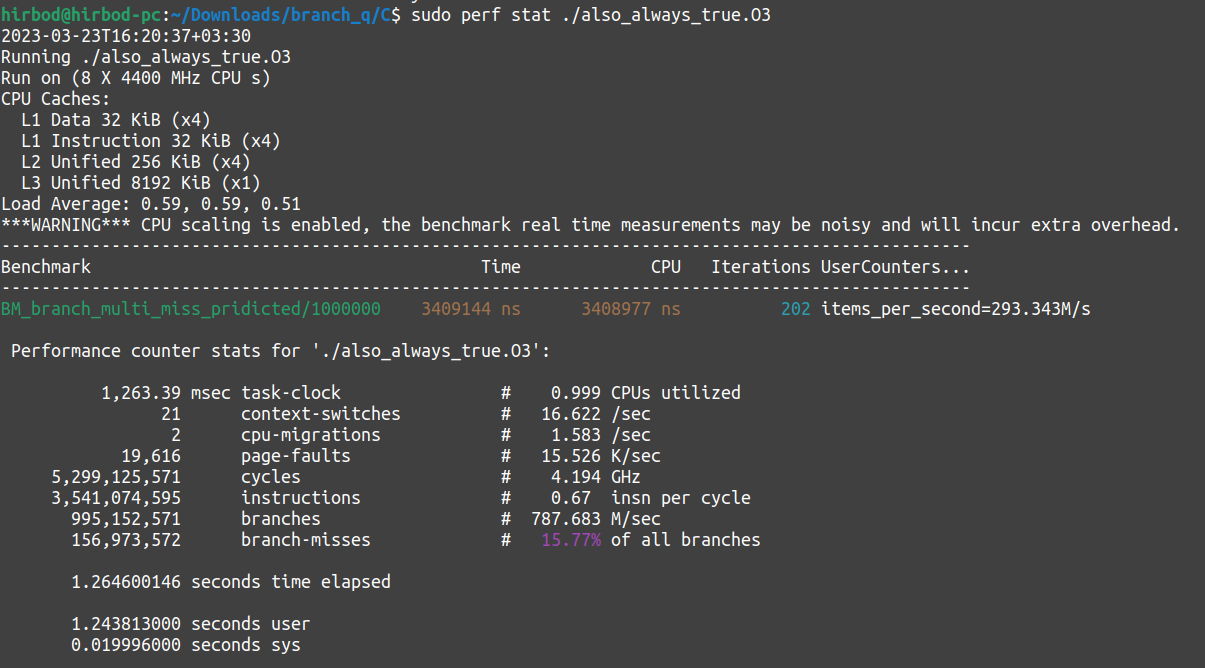
\includegraphics[scale=0.35]{pics/5/C/also_always_true.png}}
        \end{figure}
    \end{itemize}
    \end{latin}
    همان طور که مشخص است نگار که سرعت و عملکرد برنامه مثل برنامه‌ی
    \lr{pure\_random}
    در سوال قبل است. برای جواب دادن به چرایی این سوال اجازه دهید که به یک تکه کد
    C
    نگاه کنیم که تقریبا کار برنامه را انجام می‌دهد. مثل قسمت اول این تکه کد نیز به کمک godbolt
    تبدیل به assembly 
    شده است.
    \begin{figure}[H]
        \centerline{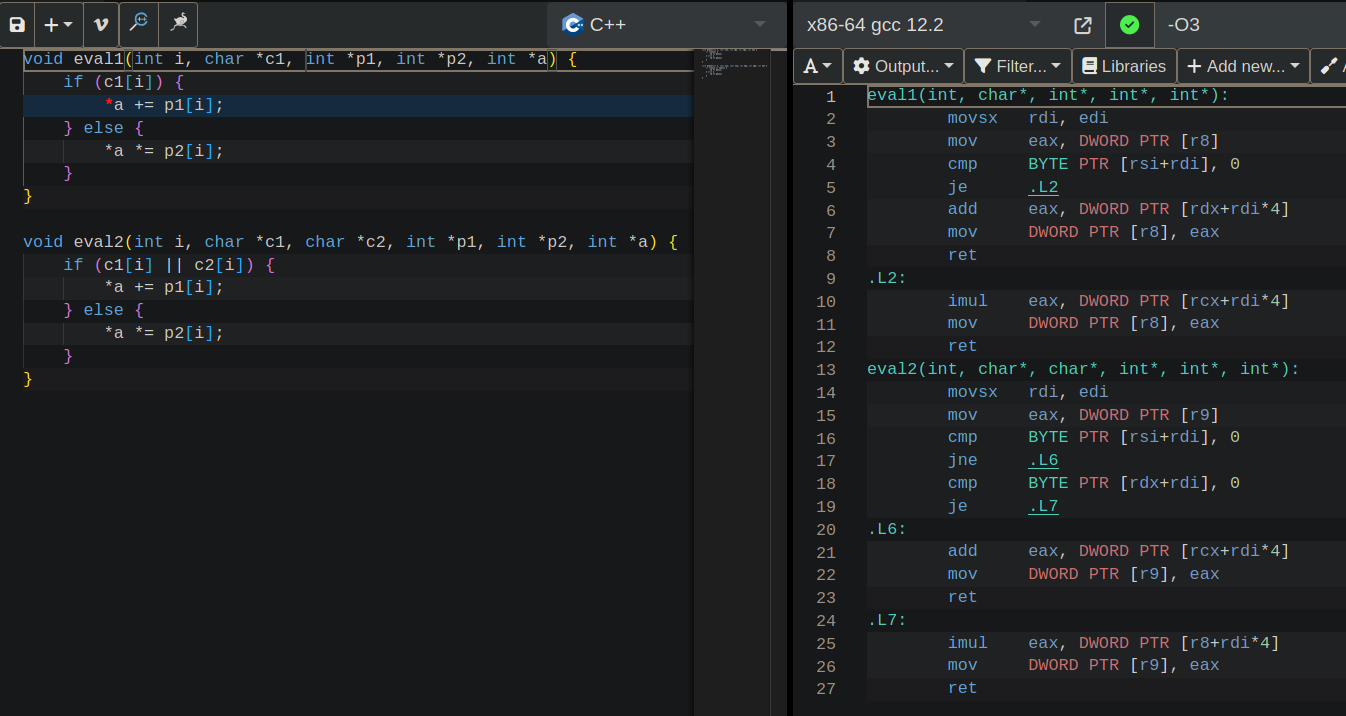
\includegraphics[scale=0.35]{pics/5/C/godbolt.png}}
    \end{figure}
    در تابع \lr{eval1}
    تنها یک branch
    وجود دارد که jump
    در صورتی اتفاق می‌افتد که
    \lr{c1[i]}
    برابر 0 باشد. از طرفی در صورتی که تابع
    \lr{eval2}
    را نگاه کنیم. متوجه می‌شویم که دو branch وجود دارد.
    در ابتدا پرش در صورتی اتفاق می‌افتد که
    \lr{c1[i]}
    غیر ۰ باشد و در صورتی که پرش اتفاق نیفتاد، چک می‌شود که آیا
    \lr{c2[i]}
    برابر ۰ است یا خیر. در صورتی که برابر ۰ باشد یک پرش رخ می‌دهد. نکته‌ای که در اینجا باید دقت کنیم
    این است که اولین
    \lr{branch}
    همیشه مقداری تصادفی دارد. برای همین پردازنده نمی‌تواند که پیش بینی کند که آیا اولین
    \lr{branch}، \lr{taken} می‌شود یا خیر.
    به صورت خلاصه‌تر و کلی دو \lr{branch}
    در اینجا وجود دارد که هر کدام به تنهایی را نمی‌توانیم پیش بینی کنیم ولی با هم می‌دانیم که همیشه
    پرش به خط ۲۱ اتفاق می‌افتد.
    \item در ابتدا بدون هیچ تغییری هر یک از برنامه‌ها را تست می‌کنیم.
    \begin{latin}
    \begin{itemize}
        \item also\_always\_true
        \begin{figure}[H]
            \centerline{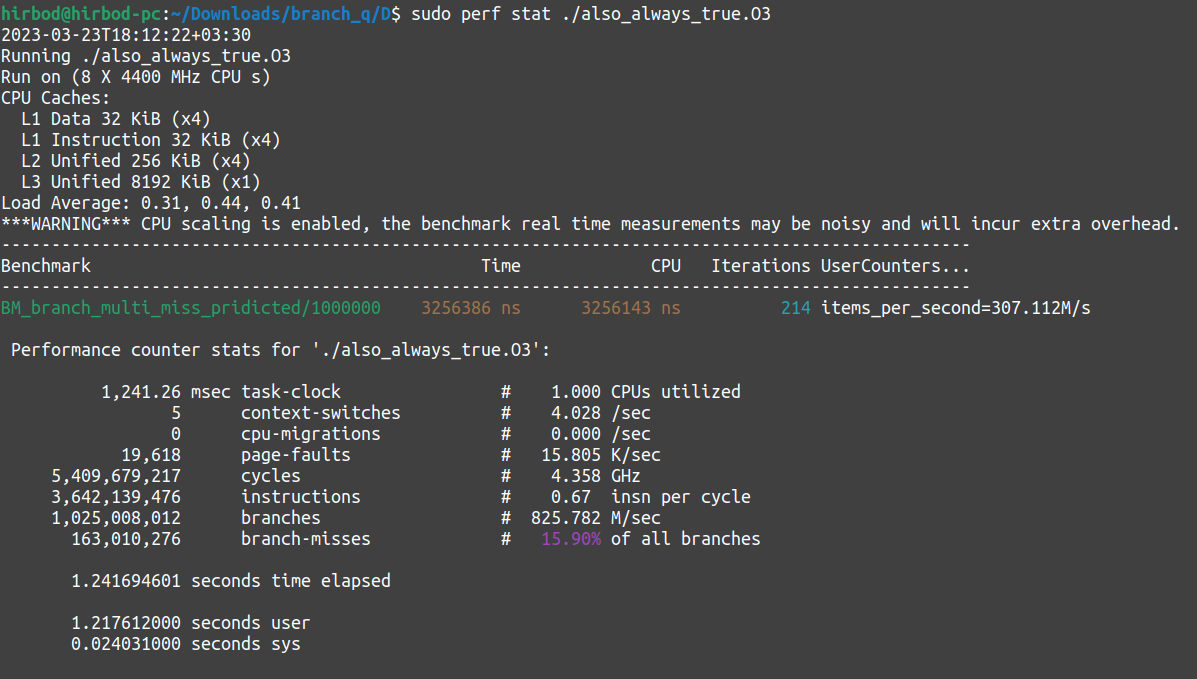
\includegraphics[scale=0.35]{pics/5/D/also_always_true.png}}
        \end{figure}
        \item pure\_random
        \begin{figure}[H]
            \centerline{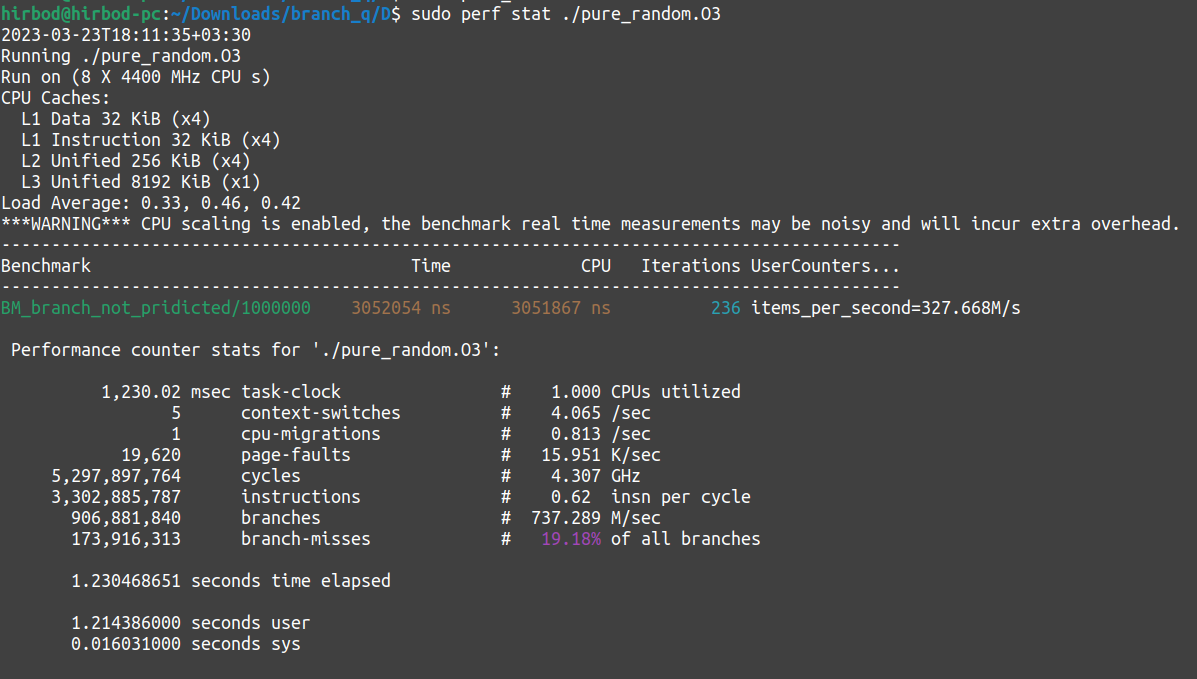
\includegraphics[scale=0.35]{pics/5/D/pure_random.png}}
        \end{figure}
        \item single\_branch
        \begin{figure}[H]
            \centerline{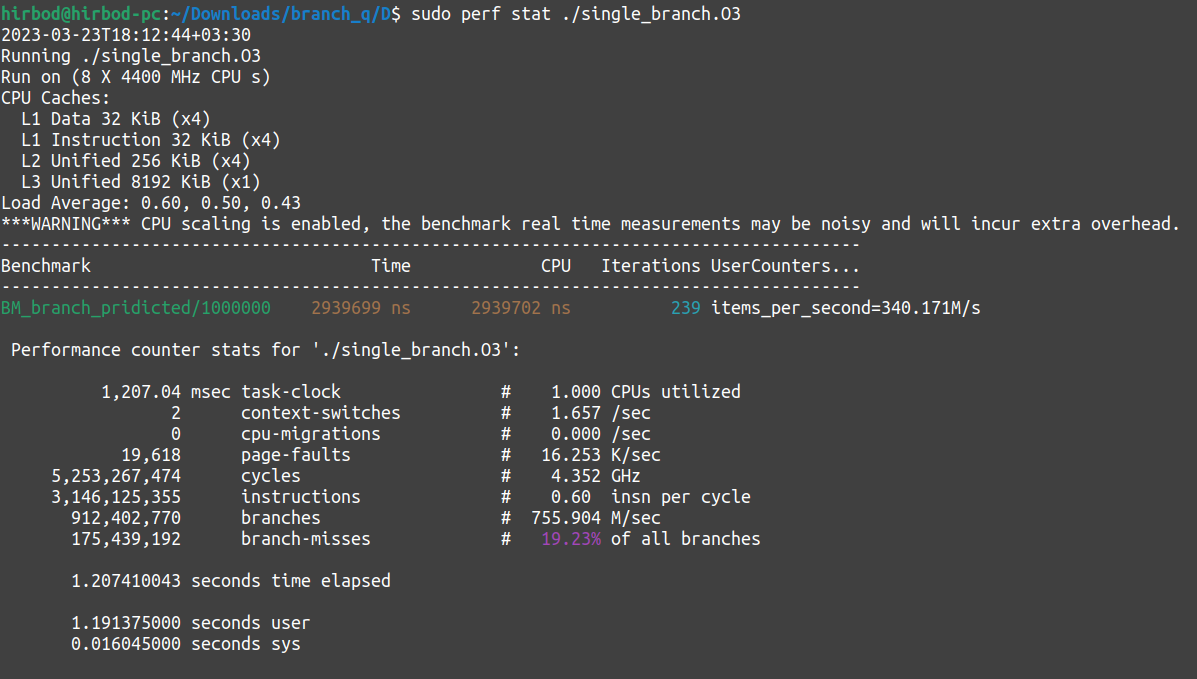
\includegraphics[scale=0.35]{pics/5/D/single_branch.png}}
        \end{figure}
    \end{itemize}
    \end{latin}
    حال بررسی می‌کنیم که هر کدام از کد‌ها را چه طور می‌توان بهبود بخشید. در فایل
    \lr{also\_always\_true}
    کافی است که به جای
    \lr{||}
    از
    \lr{|}
    استفاده کنیم. به کد اسمبلی تولید شده توجه کنید:
    \begin{figure}[H]
        \centerline{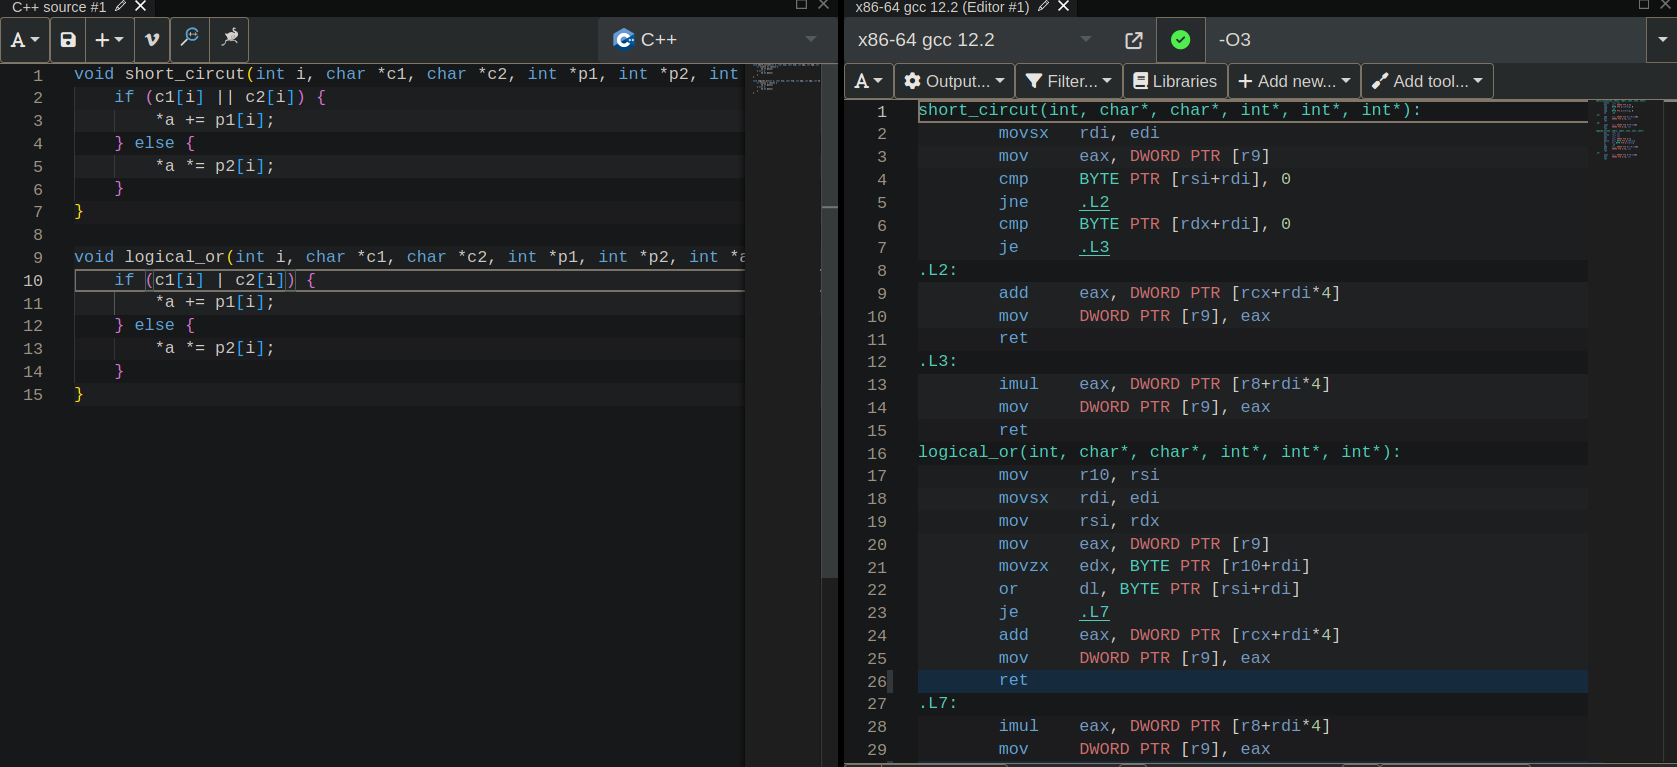
\includegraphics[scale=0.3]{pics/5/D/godbolt_also_always_true.png}}
    \end{figure}
    همان طور که در قسمت قبل هم توضیح دادیم، در تابع
    \lr{short circut}
    دو \lr{branch}
    وجود دارد که هر کدام از آنها به تنهایی به صورت رندوم عمل می‌کنند. در صورتی که از
    \lr{|}
    استفاده کنیم، به جای اینکه دو پرش اتفاق بیفتد، در ابتدا اعداد \lr{or}
    می‌شوند و سپس پرش اتفاق می‌افتد. حال به کمک perf سرعت برنامه را بررسی ‌می‌کنیم.
    \begin{figure}[H]
        \centerline{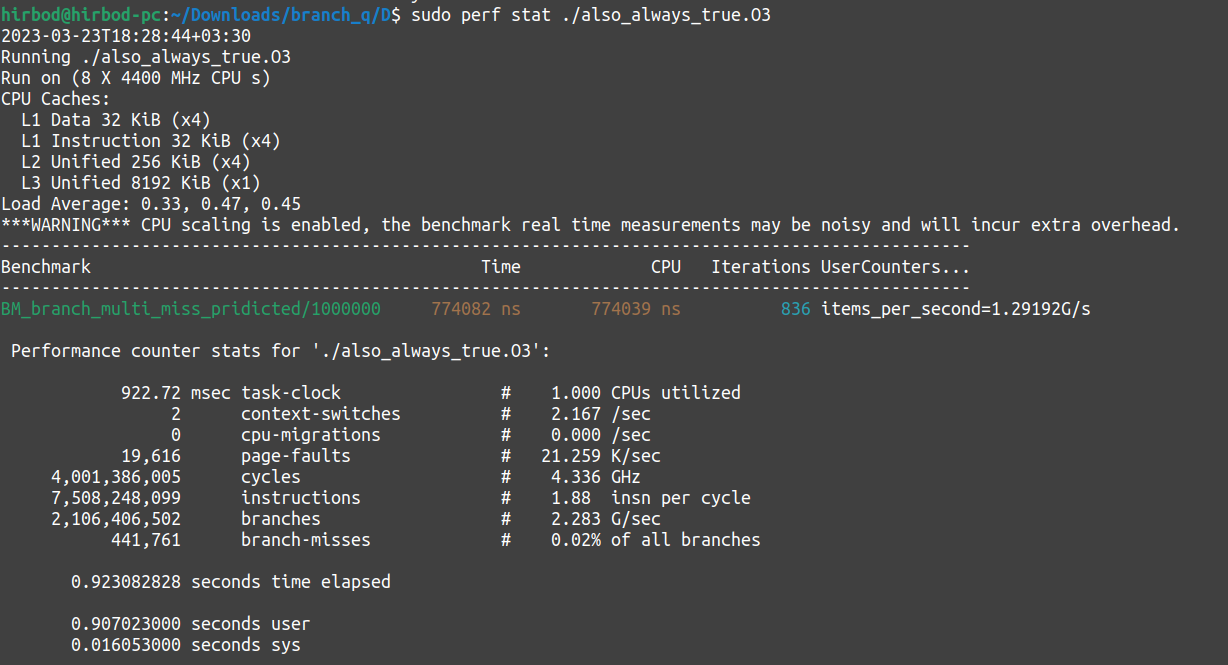
\includegraphics[scale=0.35]{pics/5/D/also_always_true_better.png}}
    \end{figure}
    همان طور که مشخص است سرعت برنامه بسیار بهتر شد و تعداد
    \lr{miss prediction}ها
    به شدت کاهش یافت.

    در ادامه به بررسی فایل
    \lr{single\_branch}
    می‌پردازیم. برای \lr{branchless}
    کردن این فایل می‌توانیم از عملیات ریاضی استفاده کنیم. کد را به صورت زیر عوض می‌کنیم:
    \codesample{codes/5D-1.cpp}
    نتیجه‌ی
    \lr{c\_ptr[i] != 0}
    یا صفر است یا یک. پس یا صفر را با $a$
    جمع می‌زنیم یا
    \lr{p1[i]}
    را. به اسمبلی کد توجه کنید:
    \begin{figure}[H]
        \centerline{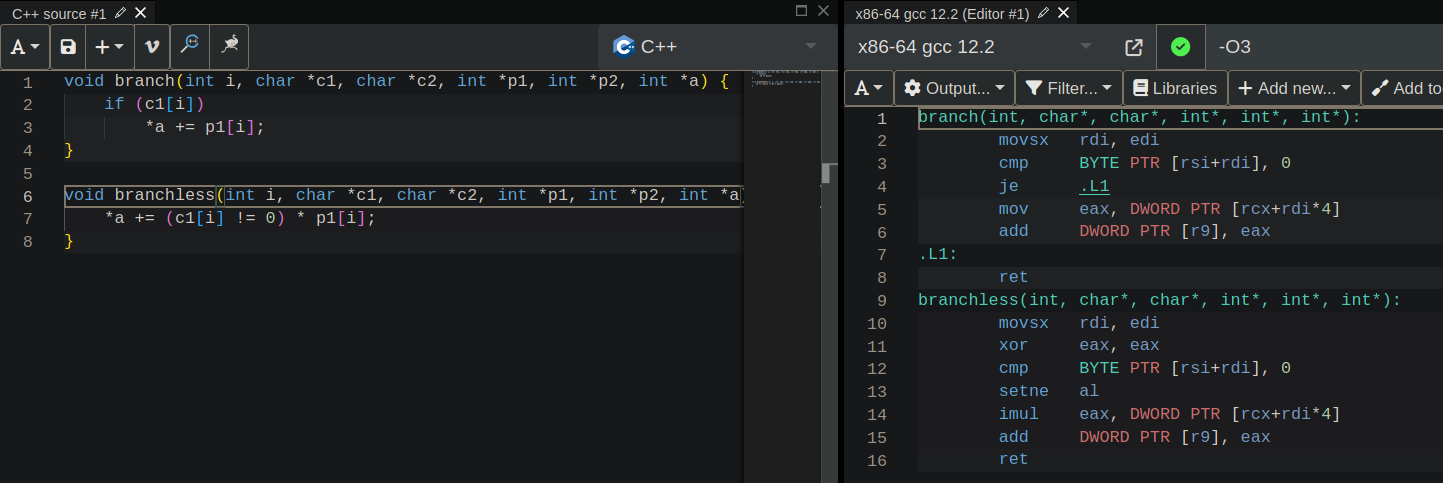
\includegraphics[scale=0.3]{pics/5/D/godbolt_single_branch.png}}
    \end{figure}
    همان طور که مشاهده می‌کنید اصلا هیچ
    \lr{branch}ی
    وجود ندارد. به کمک perf سرعت برنامه را اندازه گیری می‌کنیم:
    \begin{figure}[H]
        \centerline{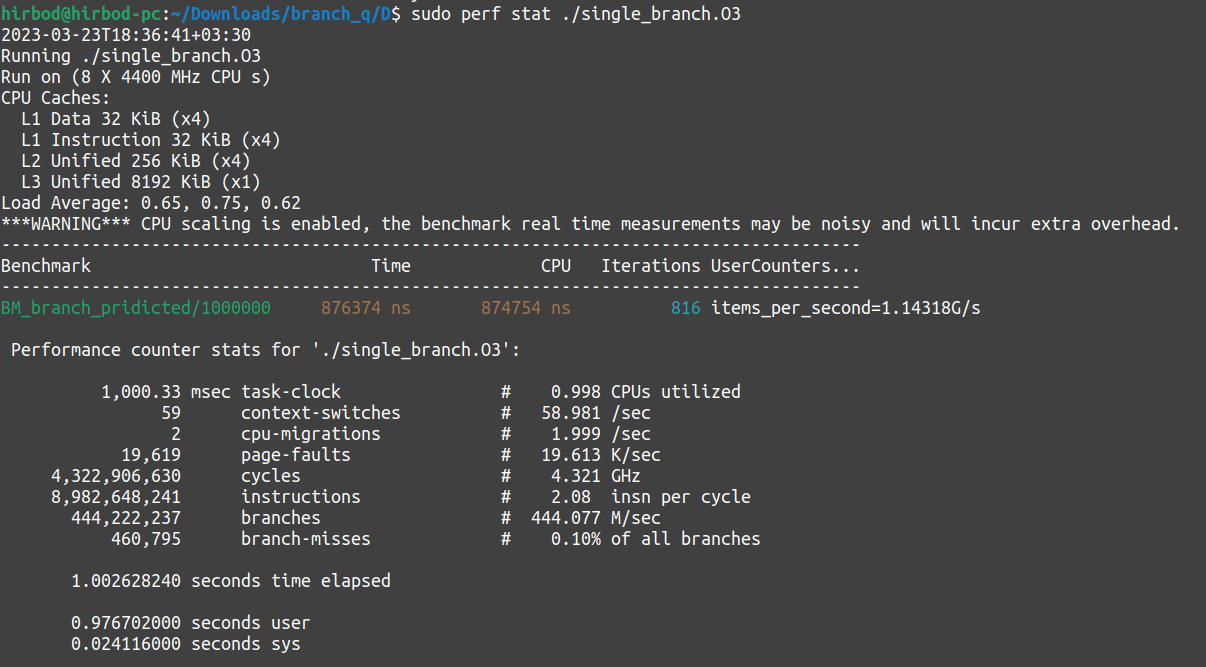
\includegraphics[scale=0.35]{pics/5/D/single_branch_better.png}}
    \end{figure}
    برای قطعه کد آخر نیز روشی مشابه با روش قسمت قبل می‌زنیم:
    \codesample{codes/5D-2.cpp}
    حال به کد اسمبلی تولید شده نگاه می‌کنیم:
    \begin{figure}[H]
        \centerline{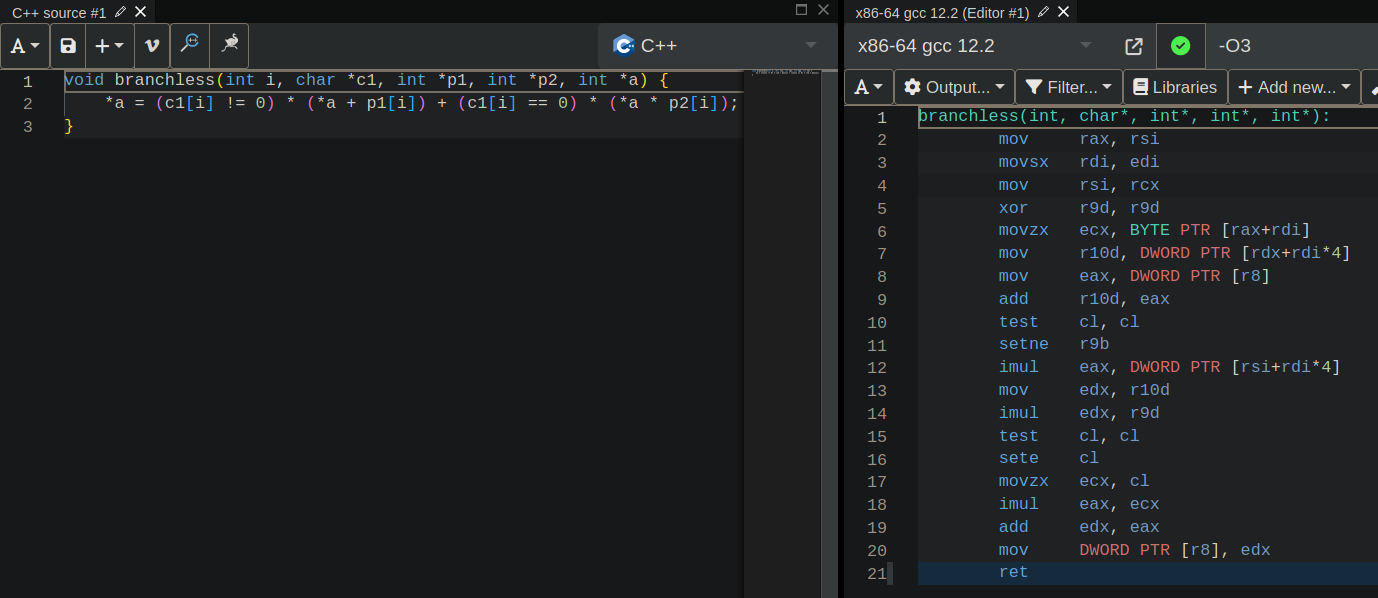
\includegraphics[scale=0.3]{pics/5/D/godbolt_pure_random.png}}
    \end{figure}
    همان طور که مشخص است هیچ
    \lr{branch}ای
    وجود ندارد. در نهایت نیز به کمک perf سرعت و تعداد \lr{missprediction}ها را بررسی می‌کنیم.
    \begin{figure}[H]
        \centerline{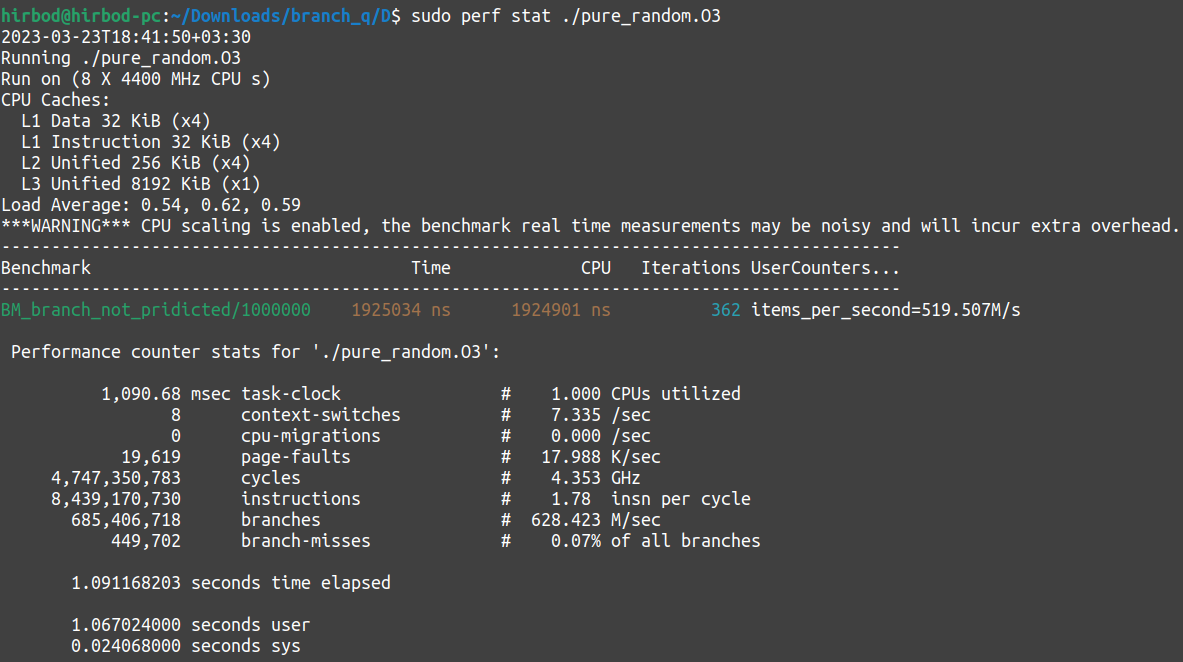
\includegraphics[scale=0.35]{pics/5/D/pure_random_better.png}}
    \end{figure}
    در نهایت باید دقت کنیم که مشکلی در اینجا به وجود آمد این بود که خوانایی کد ما به شدت کم شد!
    علاوه بر آن در بعضی از مواقع مثل زمانی که همیشه یک \lr{branch}
    درست باشد، حذف کردن \lr{branch}
    ممکن است که سربار بیشتری بر روی پردازنده قرار دهد. چرا که ممکن است که مثلا مجبور شویم
    ۱۰
    عملیات ضرب را برای حذف \lr{branch}
    انجام دهیم که این سربار زیادی را بر روی پردازنده قرار می‌دهد. ولی در صورتی که پرش‌ها کاملا تصادفی
    باشند از لحاظ
    \lr{performace}
    شاید ایده‌ی بدی نباشد که دستی
    \lr{branch}ها
    را حذف کنیم.
    \item در ابتدا مثل سوالات قبل کد‌های داده شده را بدون هیچ تغییری اجرا می‌کنیم.
    \begin{latin}
    \begin{itemize}
        \item predicted
        \begin{figure}[H]
            \centerline{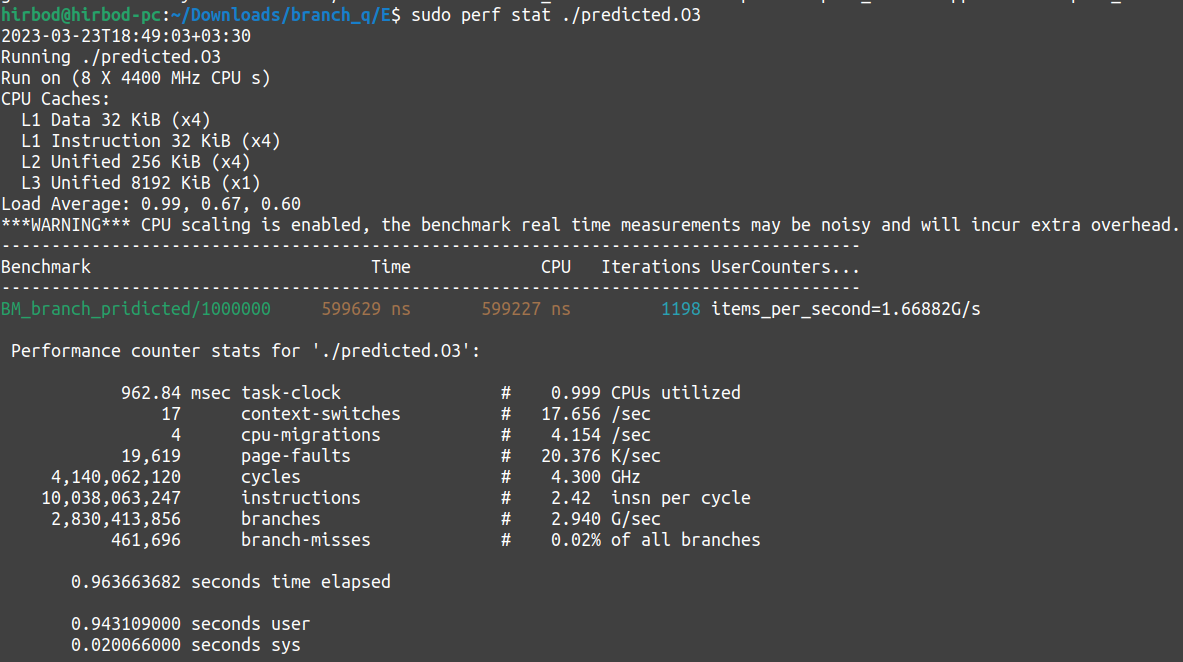
\includegraphics[scale=0.35]{pics/5/E/predicted.png}}
        \end{figure}
        \item pure\_random
        \begin{figure}[H]
            \centerline{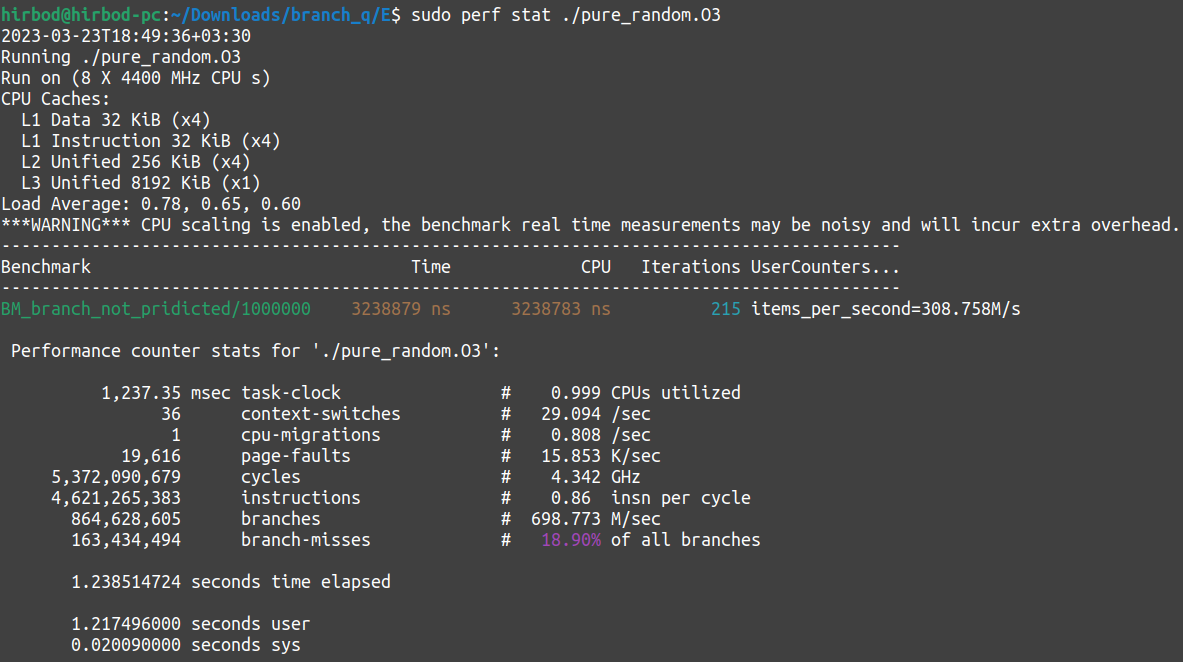
\includegraphics[scale=0.35]{pics/5/E/pure_random.png}}
        \end{figure}
    \end{itemize}
    \end{latin}
    در ابتدا فایل 
    \lr{predicted.cpp}
    را عوض می‌کنیم. داخل حلقه را به تکه کد زیر تبدیل می‌کنیم:
    \codesample{codes/5E-1.cpp}
    سپس به کمک perf
    سرعت برنامه را اندازه گیری می‌کنیم.
    \begin{figure}[H]
        \centerline{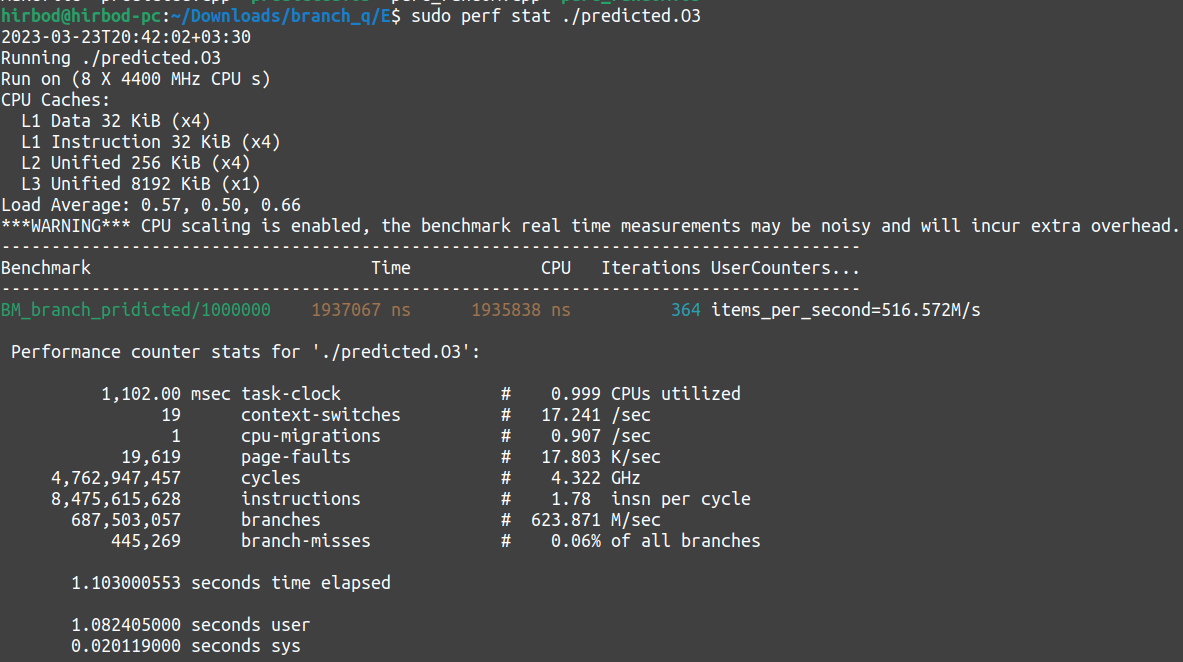
\includegraphics[scale=0.35]{pics/5/E/predicted_no_branch.png}}
    \end{figure}
    همان طور که مشاهده می‌شود سرعت برنامه به شدت کاهش یافت! حدودا ۴ برابر برنامه کند تر شد!
    دلیل این موضوع این است که در حال حاضر
    \lr{CPU}
    مجبور است که عملیات سنگین مانند سه ضرب را حتما انجام دهد.

    حال به \lr{pure random}
    می‌رسیم. در داخل حلقه را به صورت زیر تغییر می‌دهیم:
    \codesample{codes/5E-2.cpp}
    این برنامه را نیز به کمک perf
    سرعت آنرا اندازه گیری می‌کنیم.
    \begin{figure}[H]
        \centerline{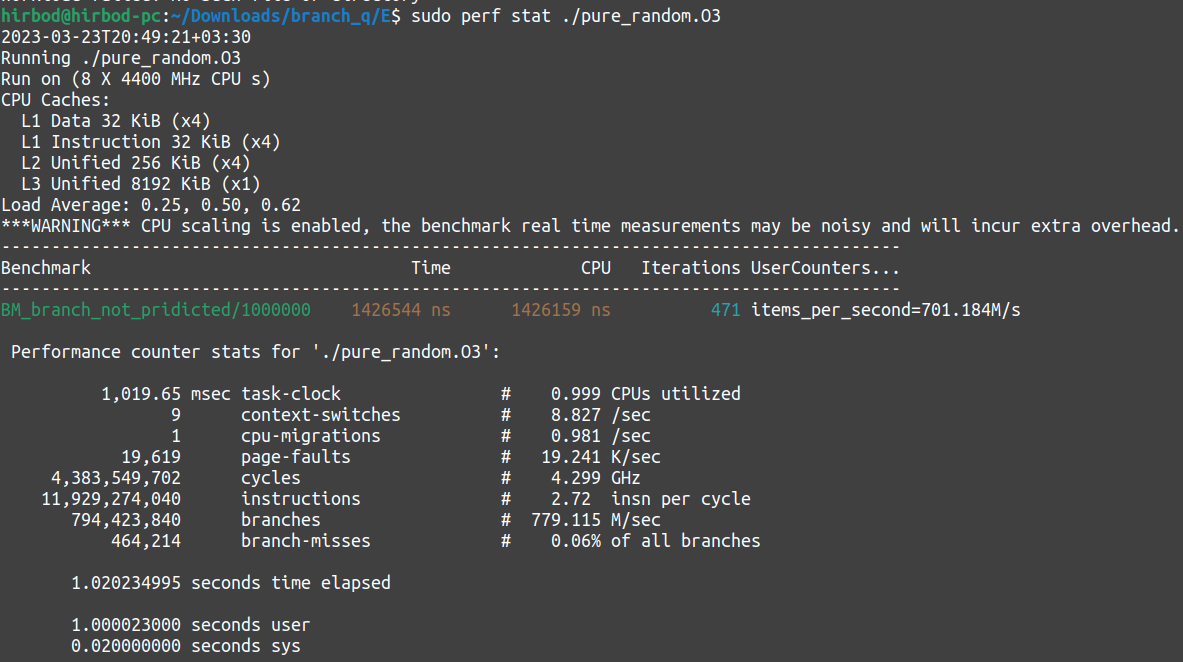
\includegraphics[scale=0.35]{pics/5/E/pure_random_no_branch.png}}
    \end{figure}
    در این قسمت ولی سرعت افزایش یافت! حدودا تعداد \lr{iteration}ها
    دو برابر شد. به نظرم سوال انتظار داشته است که سرعت این تکه کد بدون \lr{branch}
    نیز کمتر می‌شد ولی نشد. ممکن است که این موضوع به خاطر پردازنده‌ی قدیمی بنده
    (\lr{i7 4790K})
    باشد. شاید در پردازنده‌های جدیدتر روش‌های بهتری برای هندل کردن برنچ‌های تصادفی به کار رفته باشد!

    به صورت کلی برای جواب دادن به اینکه چرا کد اول کندتر شد، می‌توانیم استدلال کنیم که وسط آمدن چندین
    عملیات ضرب جدید باعث شد که سرعت برنامه کمتر شود. چرا قبل از حذف برنچ، پردازنده انتظار داشت که
    همیشه تکه کدی که add را انجام می‌داد اجرا شود (این تکه را حدس زده بود)
    و همیشه هم این
    \lr{prediction}
    درست از آب در می‌آمد. همچنین دقت کنید که add
    دستور سریعی است و در یک کلاک انجام می‌شود. اما از طرفی زمانی که به کمک ضرب،
    \lr{branch}
    را حذف کردیم، سرعت کمتر شد چرا عملا به کدی که هیچ ضربی نداشت،‌ سه عملیات ضرب اضافه کردیم و
    این باعث شد که سرعت نهایی کندتر شود.

    اما در قطعه کد دوم از آنجا که شرط به صورت رندوم اجرا می‌شد و نمی‌شد و کلی هزینه سر
    \lr{pipeline flush}
    می‌دادیم،‌ با اینکه ضرب به عبارت ما اضافه شد ولی سرعت عملیات ما بیشتر شد. چرا که دیگر نیازی به
    \lr{pipeline flush}
    نداریم.
    \item \begin{enumerate}
        \item کامپایلر ممکن است که زمانی که شرط همیشه درست یا غلط باشد به صورت کلی شرط را بردارد.
        همچنین در صورتی که با عملیات ساده و سبک (مانند and یا or)
        بتوان شرط را حذف کرد نیز این کار را انجام می‌دهد. به عنوان مثال
        \link{https://stackoverflow.com/q/11227809}{این سوال}
        را نگاه کنید که کامپایلر چه طور \lr{branch}
        را حذف می‌کند.
        \item اینکه در قبل این برنچ اتفاق افتاده است یا خیر.
        \item \lr{branch}هایی
        که \lr{pattern}های
        مشخص داشته باشند. به عنوان مثال دیدیم که دنباله‌ی
        \lr{1010101\dots}
        نیز توسط
        \lr{CPU}
        تشخیص داده شد و \lr{branch}های
        آن حدس زده می‌شد.
        \item \lr{branch}های
        متوالی که نتیجه‌ی هر کدام از آنها سخت است که حدس زده شود ولی نتیجه‌ی کلی آنها
        حدس زدنش ساده است. به عنوان مثال چند شرط تو در تو را در نظر بگیرید که به احتمال خوبی
        داخلی ترین شرط اجرا نمی‌شود ولی اینکه کجا این زنجیره متوقف می‌شود معلوم نیست.
        \item نه لزوما. بعضی وقت‌ها می‌توان کمی به
        \lr{CPU}
        کمک کرد ولی همیشه این موضوع جواب نیست. همان طور که در قسمت‌های قبل نیز گفته بودم، حداقل
        به نظر من استفاده از ضرب خیلی ایده‌ی خوبی نیست و می‌تواند که سربار زیادی را بر روی
        \lr{CPU}
        قرار دهد. در کل
        \lr{vedict}
        من این است که اول از همه باید مثل یک آدم درست حسابی و با خوانایی کد بالا کد بزنیم. سپس
        در صورت مشاهده‌ی کمبود سرعت
        \lr{critical path}های
        برنامه را پیدا کنیم و بفهمیم که چرا در آن قسمت‌ها سرعت کم می‌شود. ممکن است که اصلا مشکل
        شرط نباشد و مثلا یک
        \lr{SQL query}
        بد نوشته شده باشد!
        اگر مطمئن شده باشیم که مشکل
        \lr{branch}
        است، می‌توانیم دستی خودمان سعی ‌کنیم که آن شرط را یا حذف کنیم. دقت کنید که بعد از حذف نیز
        نیاز است که دوباره
        \lr{benchmark}
        کنیم که مثل قسمت
        \lr{E}
        نشود!

        به صورت کلی نیز کامپایلر‌ها بسیار باهوش هستند. به عنوان مثال دقت کنید که چه
        \lr{instuction}هایی
        در قطعه کد زیر تولید می‌شود:
        \begin{figure}[H]
            \centerline{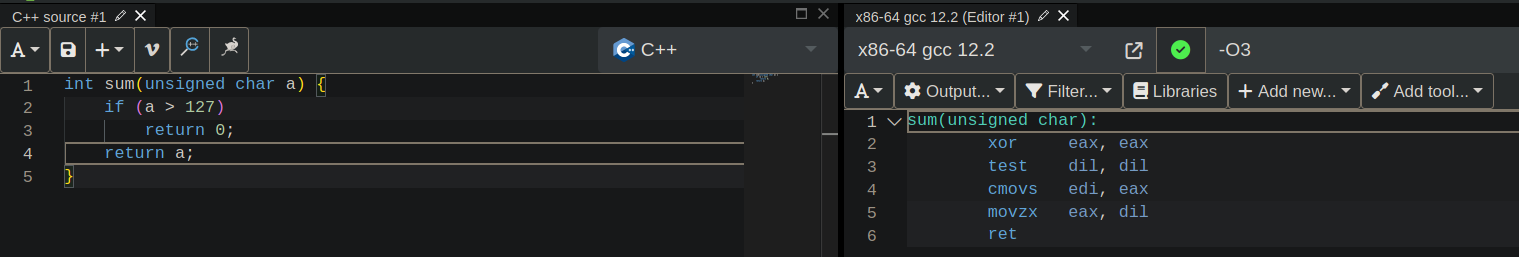
\includegraphics[scale=0.3]{pics/5/godbolt-verdict.png}}
        \end{figure}
        خود کامپایلر به قدری باهوش است که این
        \lr{branch}
        را حذف کند.
    \end{enumerate}
\end{enumerate}